\section{Simulações}

\subsection{Métodos computacionais}

Na prática, para calcular o valor da média térmica (dada pela equação \ref{eq:funcao-prob}) da magnetização (dada pela equação \ref{eq:magnetizacao2d}), seria necessário calcular a magnetização sobre todos os estados possíveis. Isso representa um notável trabalho computacional, dado que, para um grid com $N = L \times L$ spins, há $2^N$ estados possíveis.

O algoritmo de Metropolis contorna esse problema na medida em que utiliza passos de Monte Carlo para guiar a evolução do sistema. Ao invés de calcular a magnetização sobre todos os estados possíveis, a magnetização é calculada sobre estados selecionados com distribuição de probabilidade semelhante à de Gibbs (equação \ref{eq:Gibbs}). O sistema é iniciado em uma dada configuração de spins. Essa configuração pode ser aleatória ou homogênea. Um spin é, então, escolhido aleatoriamente e calcula-se a energia necessária para que esse spin seja invertido, $\delta E$. No código, um grid de spins 2D é representado por um array (matriz) $\sigma$ de formato $L \times L$ com condições periódicas de contorno e que contém valores $+1$ ou $-1$. Se o sistema se encontrava no estado $\alpha$ e mudaria para o estado $\alpha\prime$, isso significa que, de acordo com a equação \label{eq:energia}, a energia necessária para inverter o spin na posição $(i, j)$ é dada por
\begin{equation}\label{eq:deltaE}
\delta E = E_{\alpha\prime} - E_{\alpha} = 2 \sigma_{i, j} \left[J \left(\sigma _{i - 1, j} + \sigma _{i + 1, j} + \sigma _{i, j - 1} + \sigma _{i, j + 1}\right) + h\right]\text{.}
\end{equation} 
Caso essa mudança reduza a energia do sistema, isto é, $\delta E \leq 0$, o spin é invertido e o sistema é levado, consequentemente, a outro microestado. Caso contrário, o spin é invertido ou não de acordo com uma distribuição probabilística dada pela equação \ref{eq:probabilidade}. Isso é feito obtendo-se um número de forma aleatória com distrubição de probabilidade uniforme no intervalo $[0, 1]$. Se esse número for maior do que $P_{\text{flip}}$ (a probabilidade do sistema mudar do estado $\alpha$ para o estado $\alpha\prime$), o spin não é invertido. Caso contrário, o sistema também é levado ao estado $\alpha\prime$. Em seguida, é escolhido outro spin (que não havia sido escolhido previamente) aleatoriamente e o mesmo procedimento para inverter ou não o spin; e esse processo é repetido após $N_{\text{steps}}$ passos.

Para cada passo de Monte Carlo, é possível calcular a magnetização do microestado correspondente através da equação \ref{eq:magnetizacao-2d}. Dessa forma, ao fim de $N_{\text{steps}}$ passos, a magnetização é calculada como a média sobre os valores de magnetização simulados:
\begin{equation}\label{eq:magnetizacao-simulacao}
\langle m \rangle = \frac{1}{N_{\text{steps}}} \sum _{\alpha \in \text{var}} m_{\alpha}\text{.}
\end{equation}
A energia média ($e$) é calculada de forma análoga.

A figura \ref{fig:evolucao-grid-100x100} esquematiza as configurações inicial e final de um grid com $100 \times 100$ spins com condições periódicas de contorno sem campo magnético externo ($h = 0$) à temperatura $T = 1$. Para este exemplo, foram realizados $2000$ passos de Monte Carlo na simulação através do algoritmo de Metropolis. O sistema é iniciado com uma configuração de spins aleatória e atinge um estado final com regiões compactas de mesma magnetização.

\begin{figure}[ht]
	\centering
	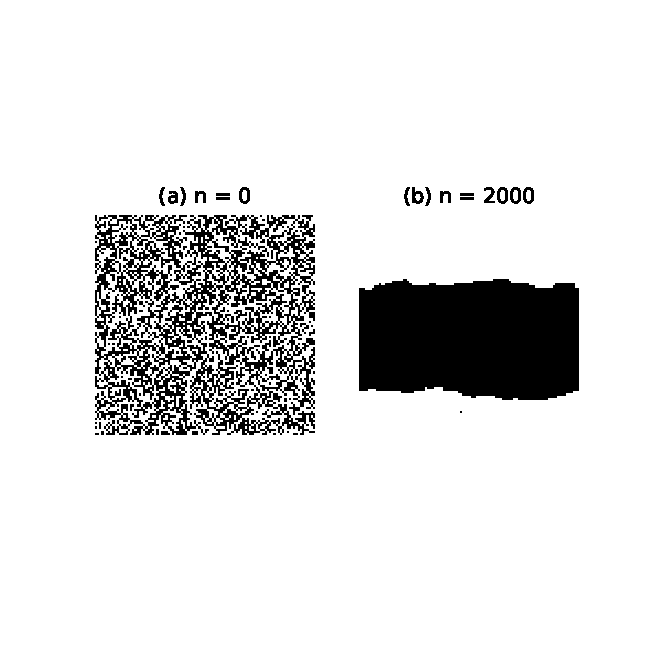
\includegraphics[scale = 1]{./img/evolucao-grid-100x100}
    \caption{Configurações inicial (esquerda) e final após $2000$ passos de Monte Carlo (direita) de um grid com $100 \times 100$ spins com condições periódicas de contorno e $J = 1$, $h = 0$ e $T/k_B = 1$.}
    \label{fig:evolucao-grid-100x100}
\end{figure}

Nas simulações deste trabalho, foi fixado o valor da constante de Boltzmann em $k_B = 1$.\footnote{Uma outra forma de entender isso é pensar que a temperatura é dada em unidades de $\left[T\right] / \left[k_B\right]$.}

\subsection{Resultados}

A figura \ref{fig:evolucao-mc-temperaturas} mostra a evolução da magnetização por sítio e da energia por sítio para um grid com $100 \times 100$ spins com condições periódicas de contorno e $J = 1$ e $h = 0$ a cada passo de Monte Carlo para alguns valores de temperatura próximos à temperatura \ref{eq:temp-crit}. É possível notar que o sistema pode levar alguns passos de Monte Carlo para atingir valores estacionários de magnetização por sítio e de energia por sítio em função da temperatura, isto é, há um comportamento de transição (transiente). Para temperaturas mais baixas, o sistema atinge valores estacionários mais rapidamente.

\begin{figure}[ht]
	\centering
	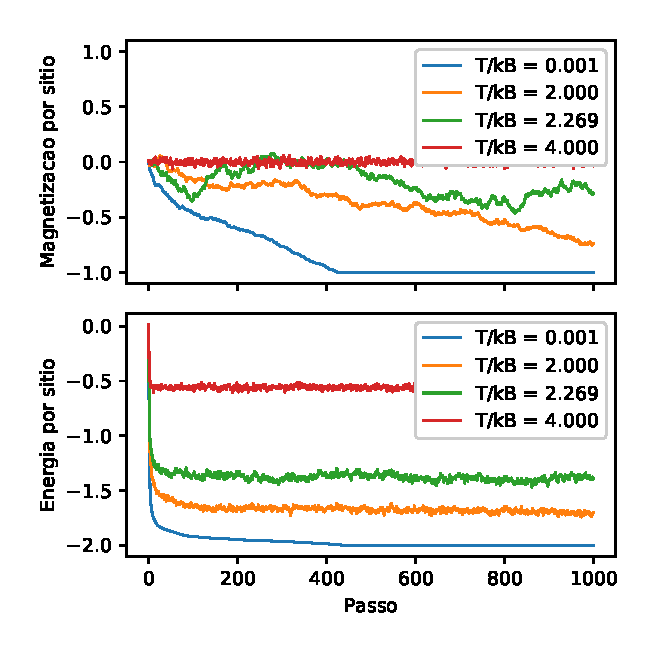
\includegraphics[scale = 1]{./img/evolucao-mc-temperaturas}
    \caption{Evolução da magnetização por sítio (acima) e da energia por sítio (abaixo) de um grid com $100 \times 100$ spins com condições periódicas de contorno e $J = 1$ e $h = 0$ a cada passo de Monte Carlo para alguns valores de temperatura próximos à temperatura crítica (equação \ref{eq:temp-crit}).}
    \label{fig:evolucao-mc-temperaturas}
\end{figure}

A figura \ref{fig:simulacao-3-larguras} mostra as curvas de magnetização por sítio médias e de energia por sítio médias de simulações com 

\begin{figure}[ht]
	\centering
	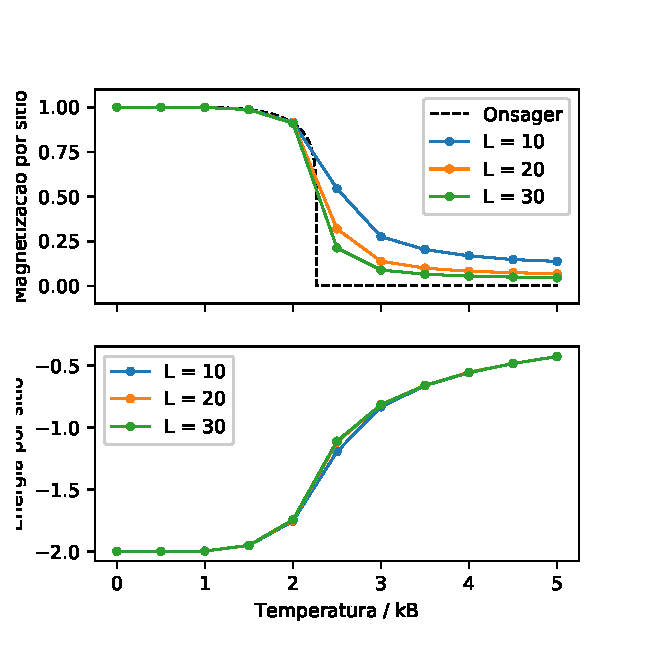
\includegraphics[scale = 1]{./img/simulacao-3-larguras}
    \caption{Curvas de magnetização por sítio (acima) e energia por sítio (abaixo) em função da temperatura de grids com $10 \times 10$, $20 \times 20$ e $30 \times 30$ spins com condições periódicas de contorno e $J = 1$ e $h = 0$.}
    \label{fig:simulacao-3-larguras}
\end{figure}

\begin{figure}[ht]
	\centering
	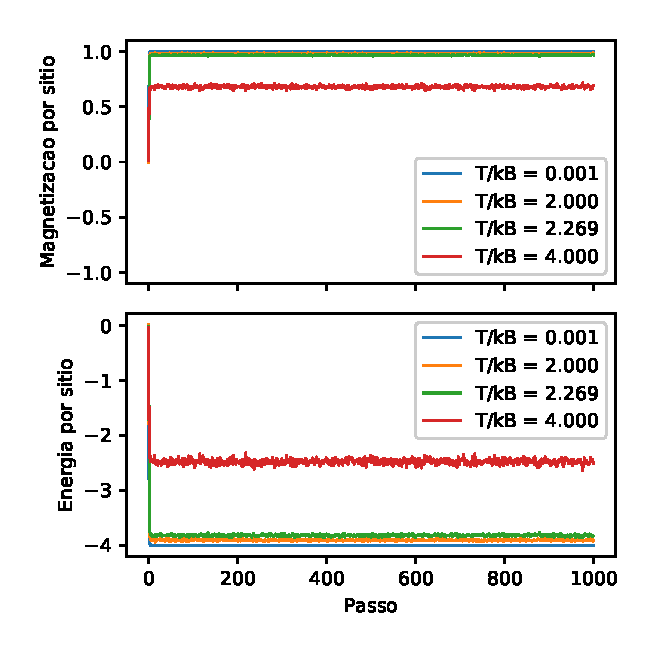
\includegraphics[scale = 1]{./img/evolucao-h=1-mc-temperaturas}
    \caption{Evolução da magnetização por sítio (acima) e da energia por sítio (abaixo) de um grid com $100 \times 100$ spins com condições periódicas de contorno e $J = 1$ e $h = 1$, a cada passo de Monte Carlo, para alguns valores de temperatura próximos à temperatura crítica (eq).}
    \label{fig:evolucao-h=1-mc-temperaturas}
\end{figure}

\begin{figure}[ht]
	\centering
	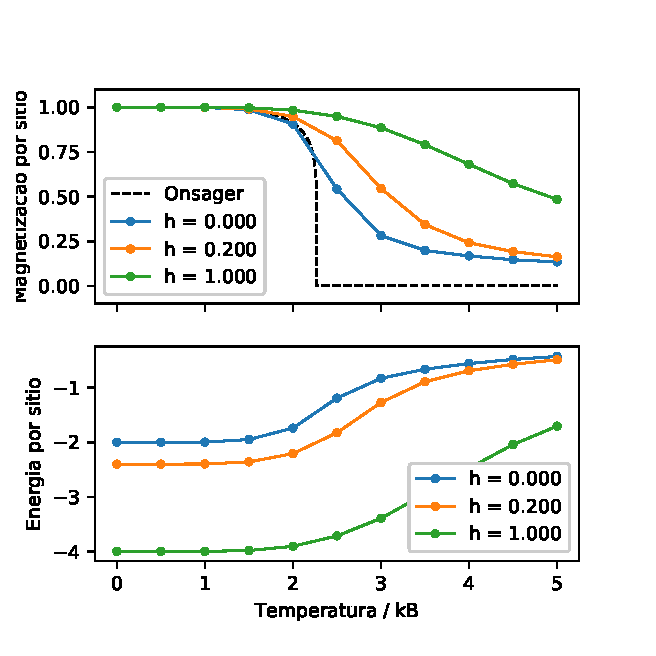
\includegraphics[scale = 1]{./img/simulacao-h}
    \caption{Curvas de magnetização por sítio (acima) e energia por sítio (abaixo) em função da temperatura de um grid com $10 \times 10$ spins com condições periódicas de contorno e $J = 1$ e $h = 0$, $0.2$ e $1$.}
    \label{fig:simulacao-h}
\end{figure}